% Introducción
{\setbeamertemplate{background}{

\includegraphics[width=\the\paperwidth,height=\the\paperheight]{images/White.png}}
\begin{frame}
  \frametitle{Introducción}
  \framesubtitle{Problemas de visibilidad.} %%Subtítulo de la diapositiva (opcional)
  Determinar regiones de visibilidad de un objeto geométrico bajo restricciones es
  un problema muy estudiado en \textit{Geometría Computacional}.
  
  \centering 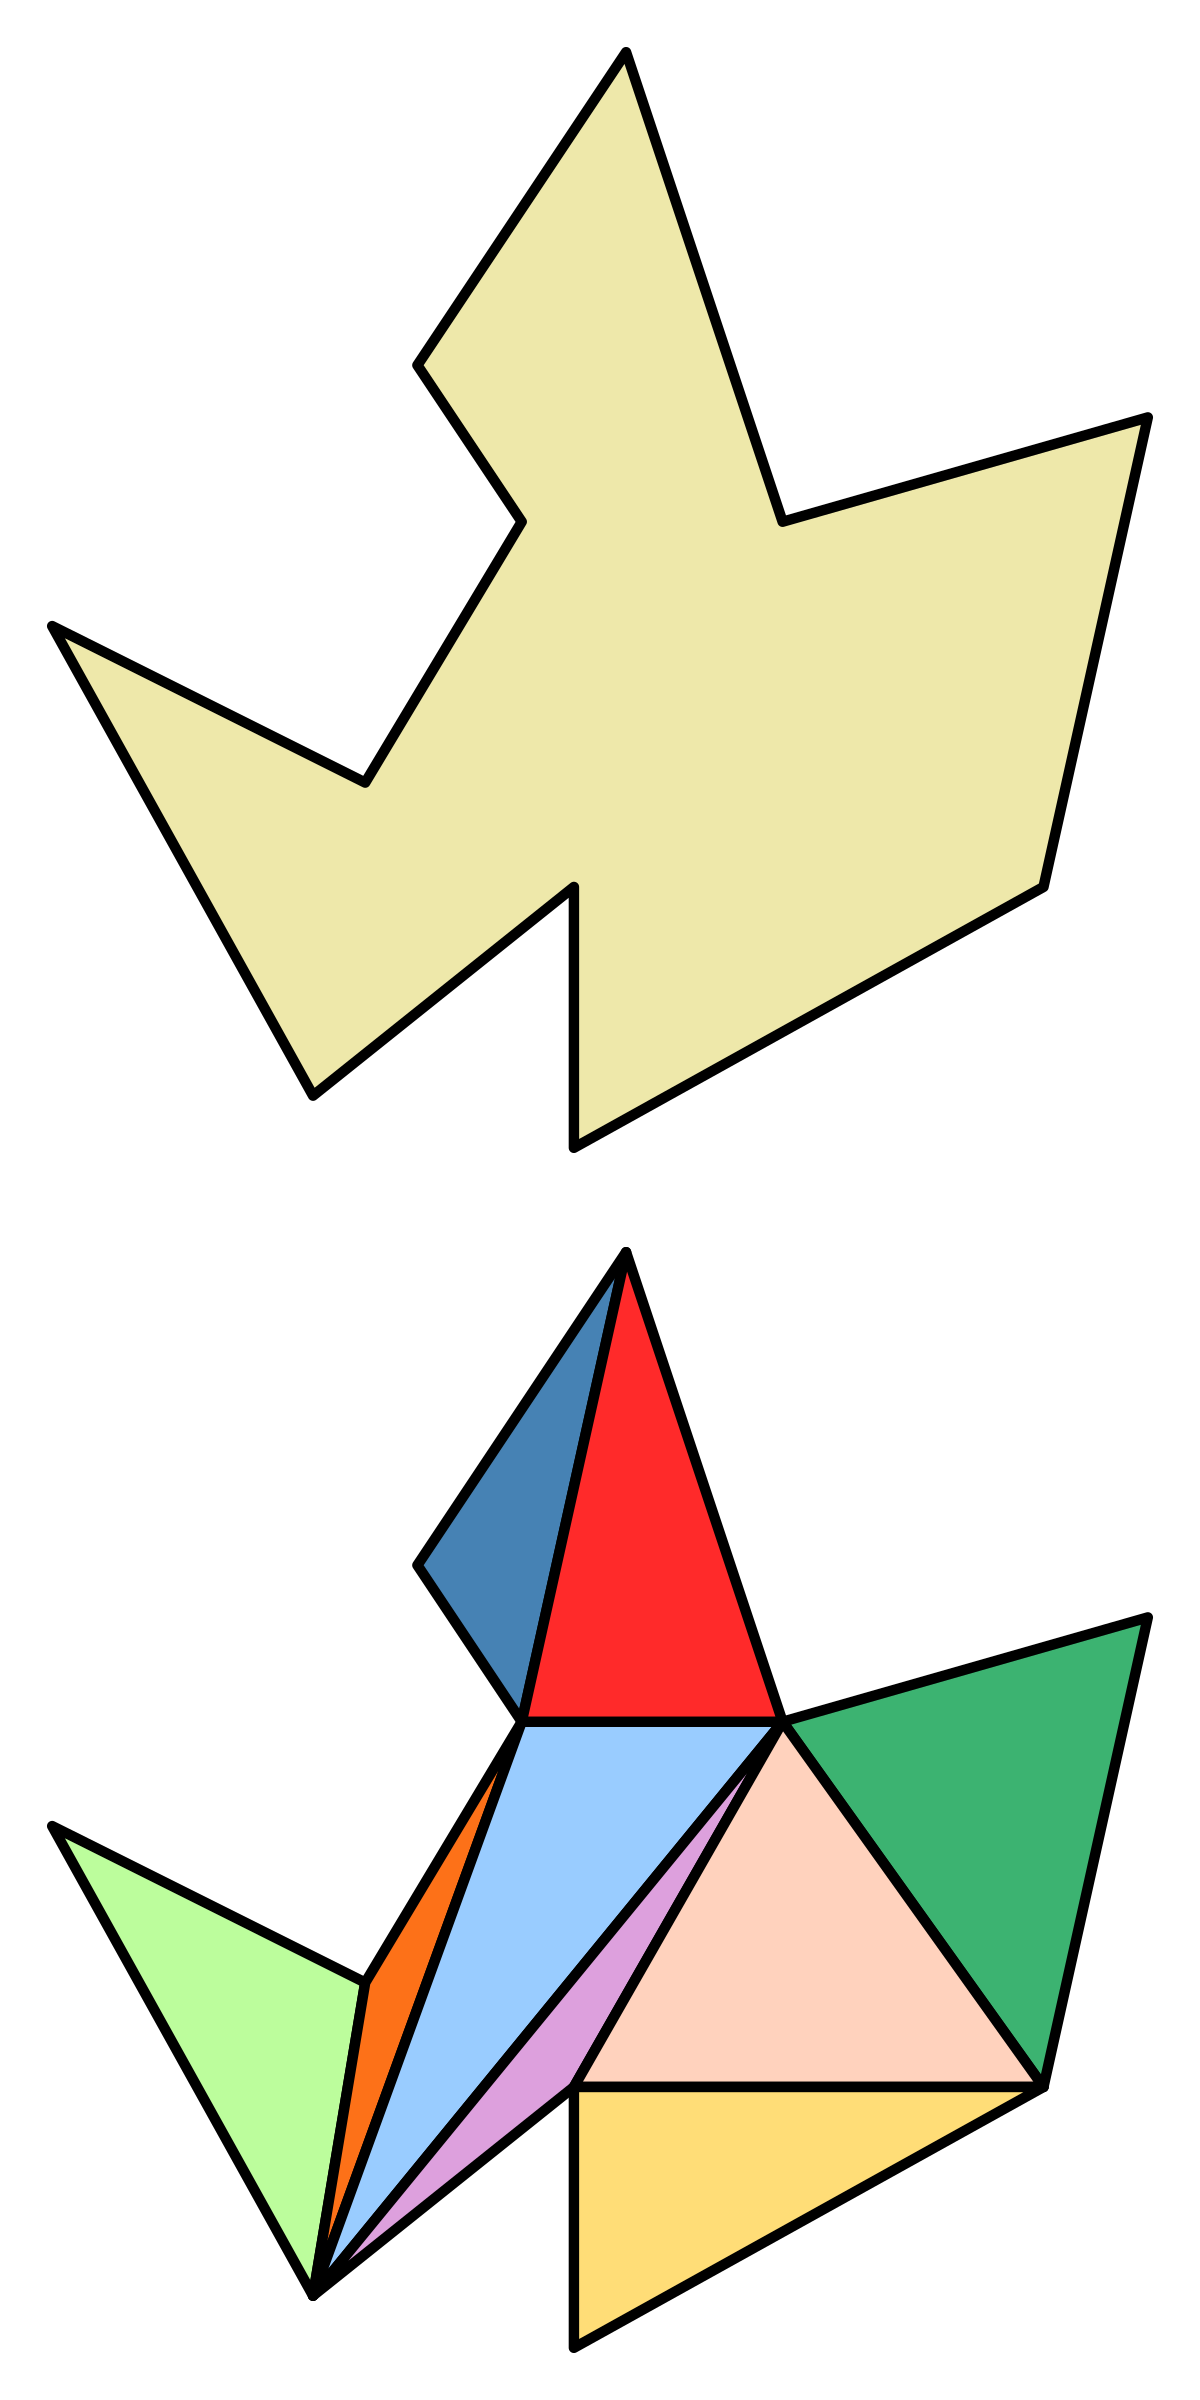
\includegraphics[width=0.15 \paperwidth]{images/Visibility.png}
\end{frame}

\begin{frame}
  \frametitle{Introducción}
  \framesubtitle{Polígono de visibilidad.} %%Subtítulo de la diapositiva (opcional)
  Definimos un \underline{Polígono de visibilidad} como el polígono formado a partir
  de un punto $q$ dentro de un polígono dado, digamos $P$. Entonces, el polígono
  de visibilidad de $q$ definido como
  \[V(q) = \{p \in P\ \big|\ q \text{ visualiza a } p\}.\]
\end{frame}

\begin{frame}
  \centering 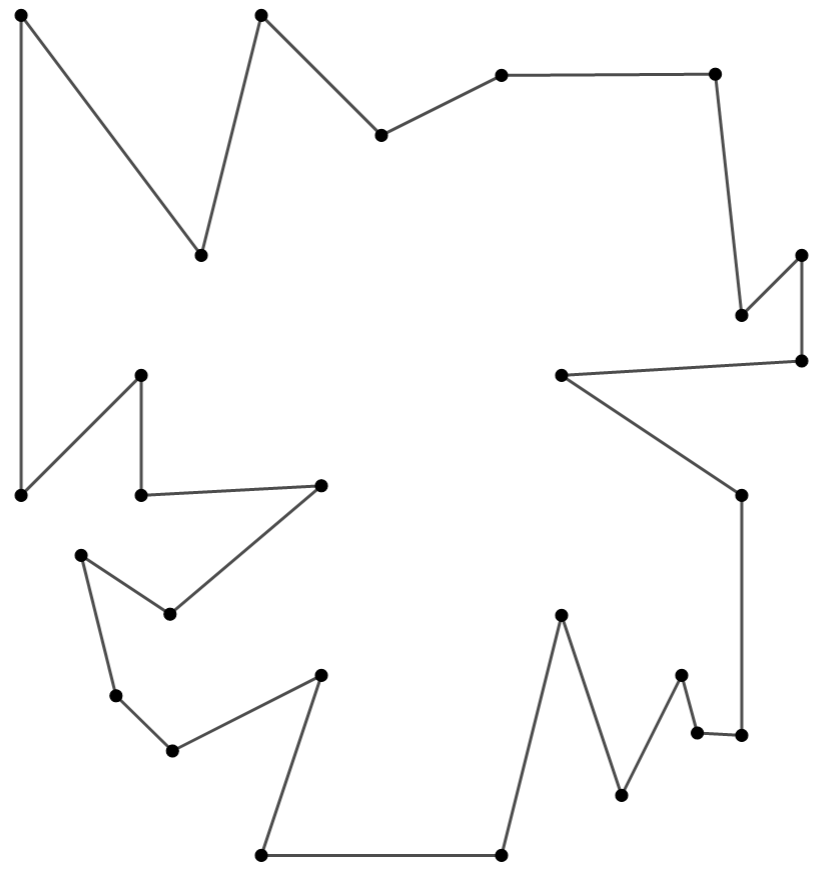
\includegraphics[width=0.55 \paperwidth]{images/V(q)01.png}
\end{frame}

\begin{frame}
  \centering 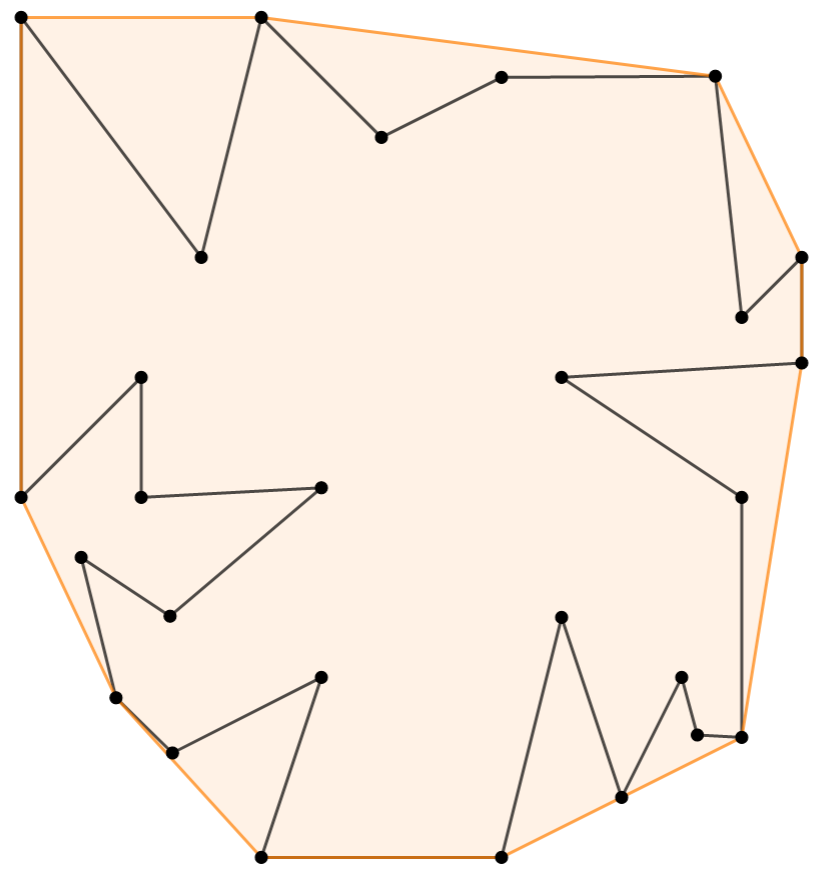
\includegraphics[width=0.55 \paperwidth]{images/V(q)02.png}
\end{frame}

\begin{frame}
  \centering 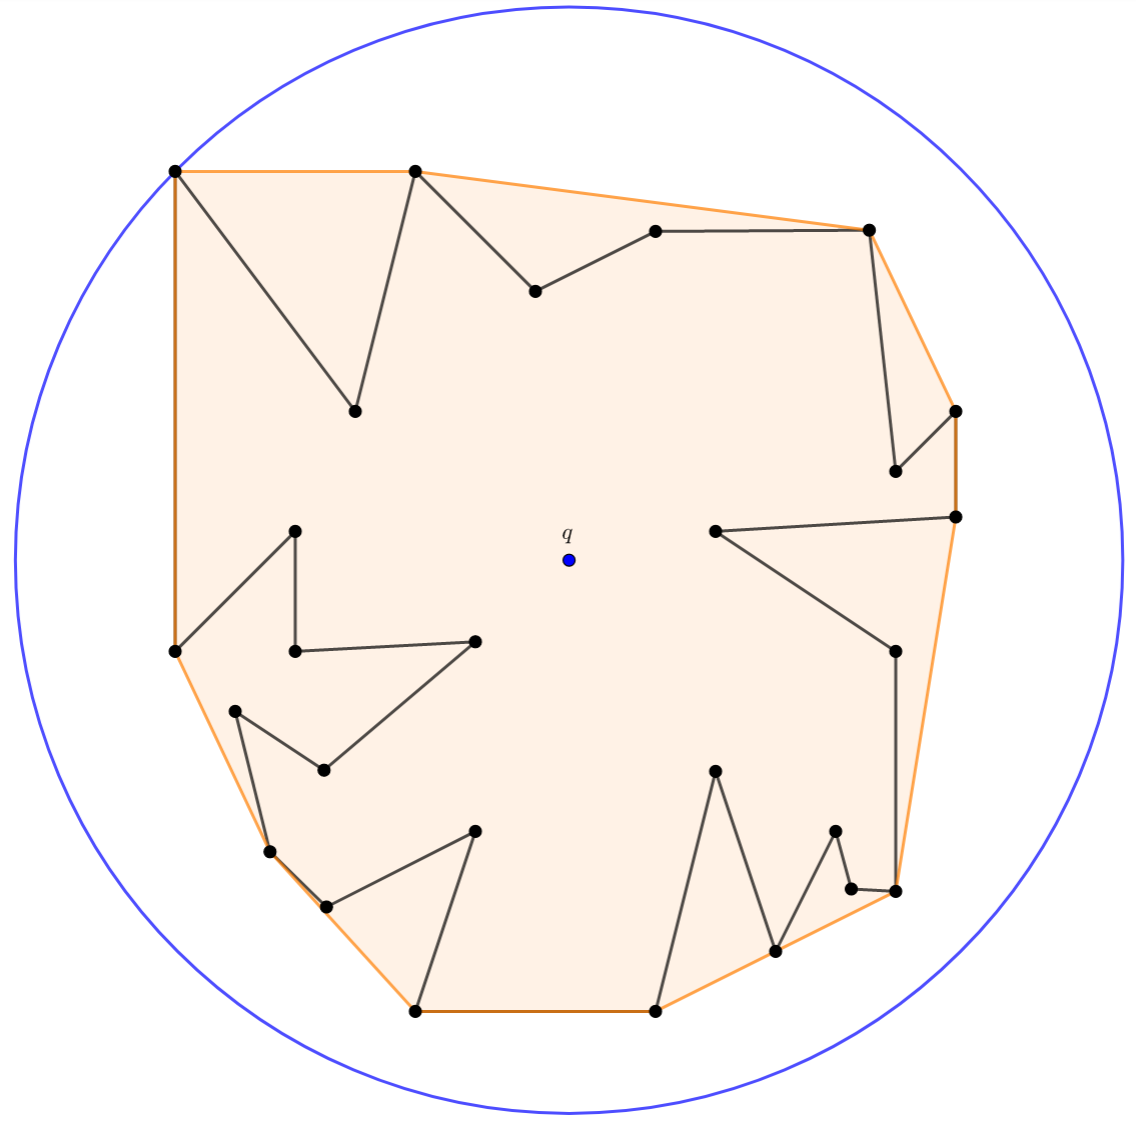
\includegraphics[width=0.55 \paperwidth]{images/V(q)03.png}
\end{frame}

\begin{frame}
  \centering 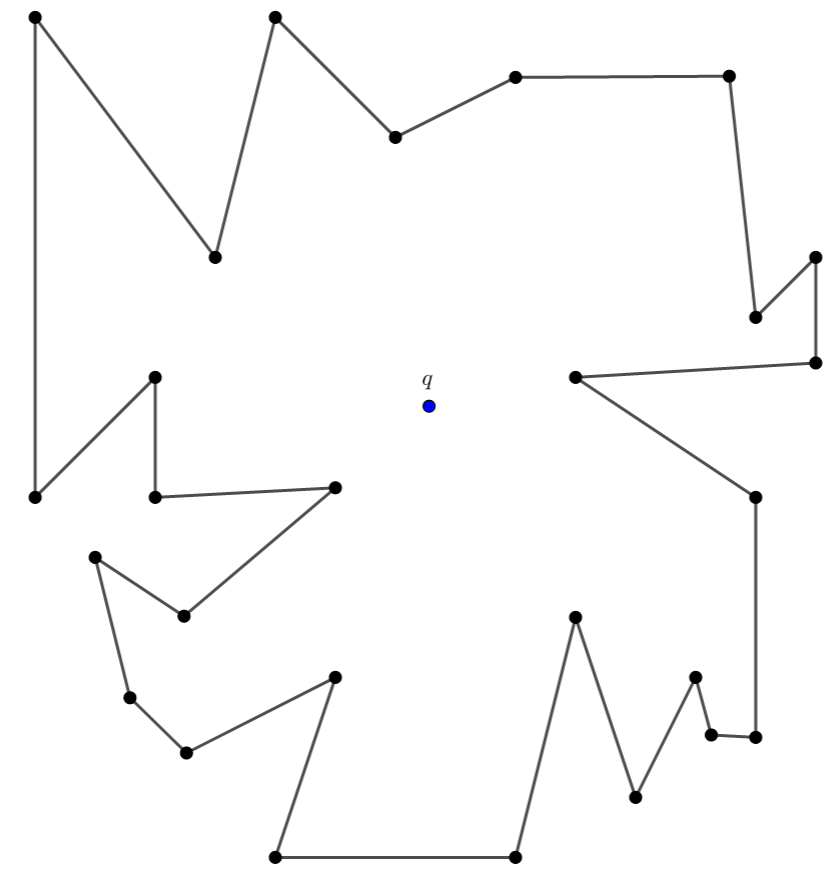
\includegraphics[width=0.55 \paperwidth]{images/V(q)04.png}
\end{frame}

\begin{frame}
  \centering 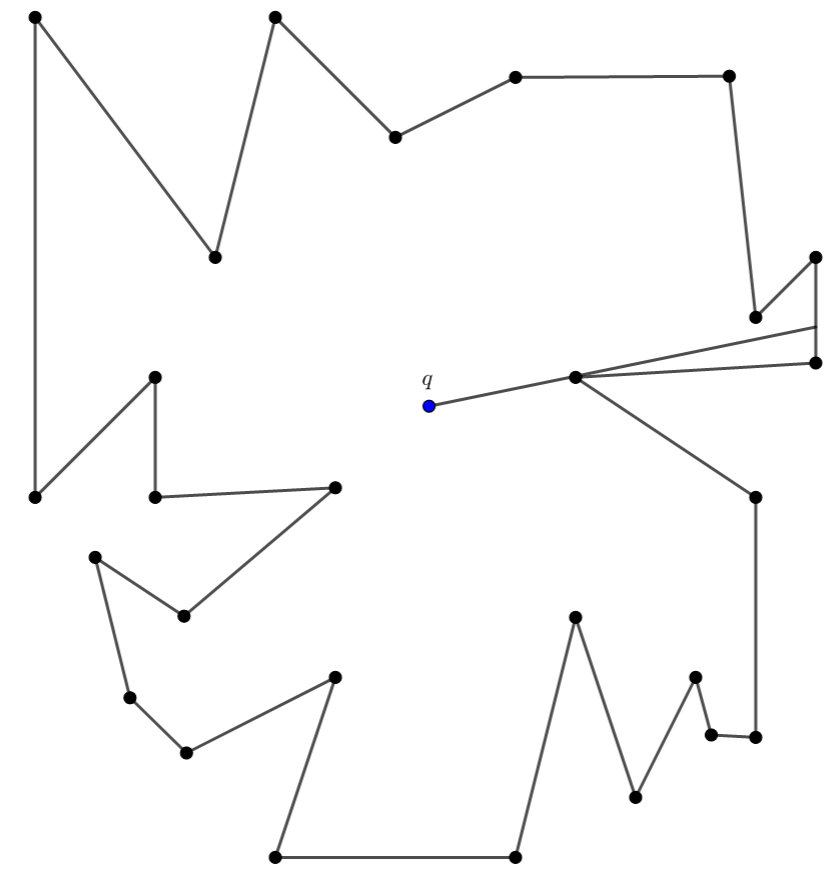
\includegraphics[width=0.55 \paperwidth]{images/V(q)05.png}
\end{frame}

\begin{frame}
  \centering 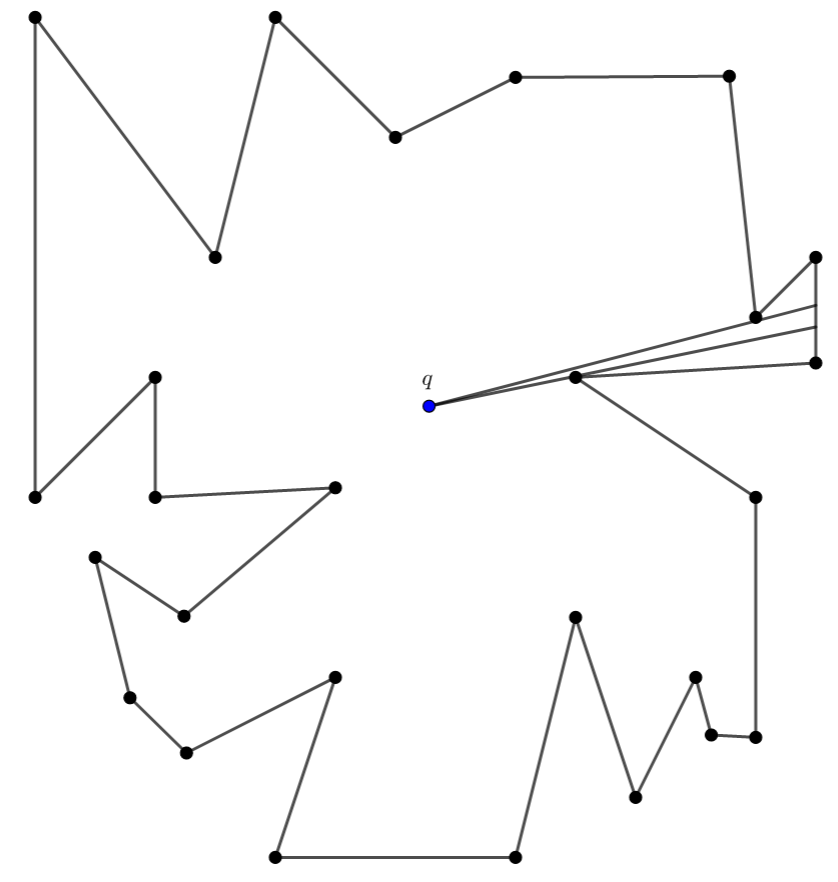
\includegraphics[width=0.55 \paperwidth]{images/V(q)06.png}
\end{frame}

\begin{frame}
  \centering 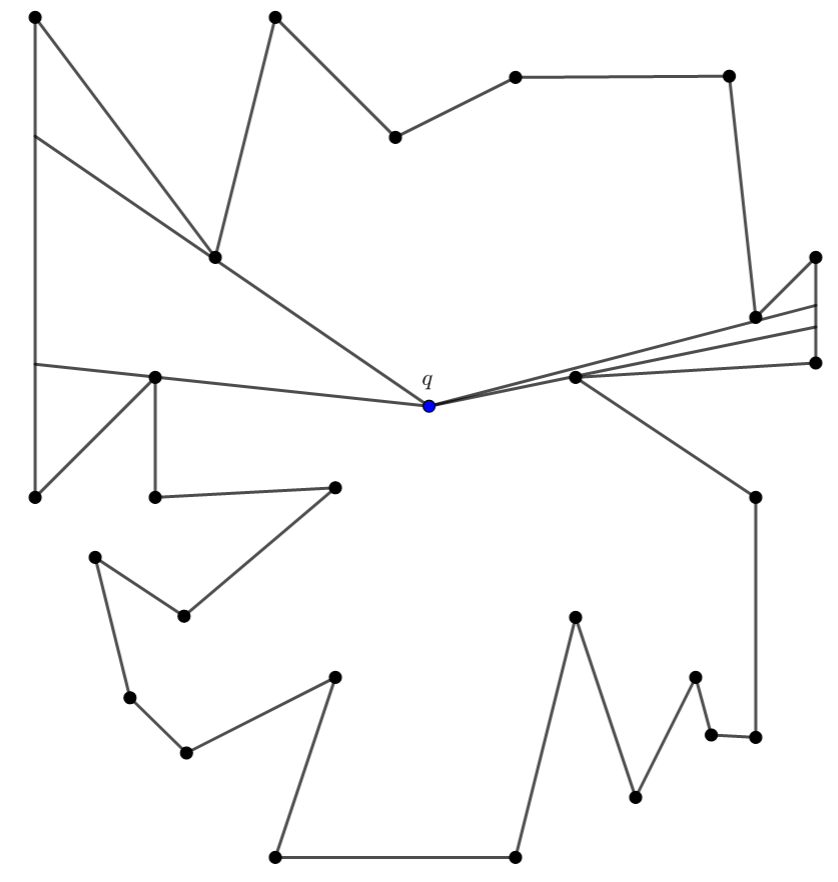
\includegraphics[width=0.55 \paperwidth]{images/V(q)07.png}
\end{frame}

\begin{frame}
  \centering 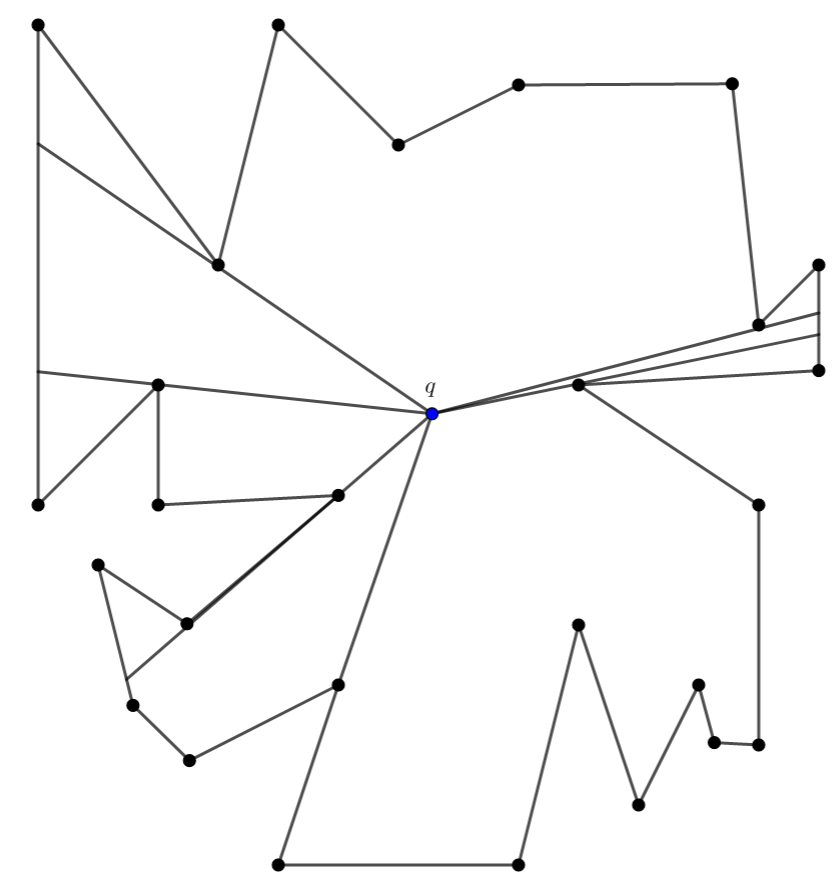
\includegraphics[width=0.55 \paperwidth]{images/V(q)08.png}
\end{frame}

\begin{frame}
  \centering 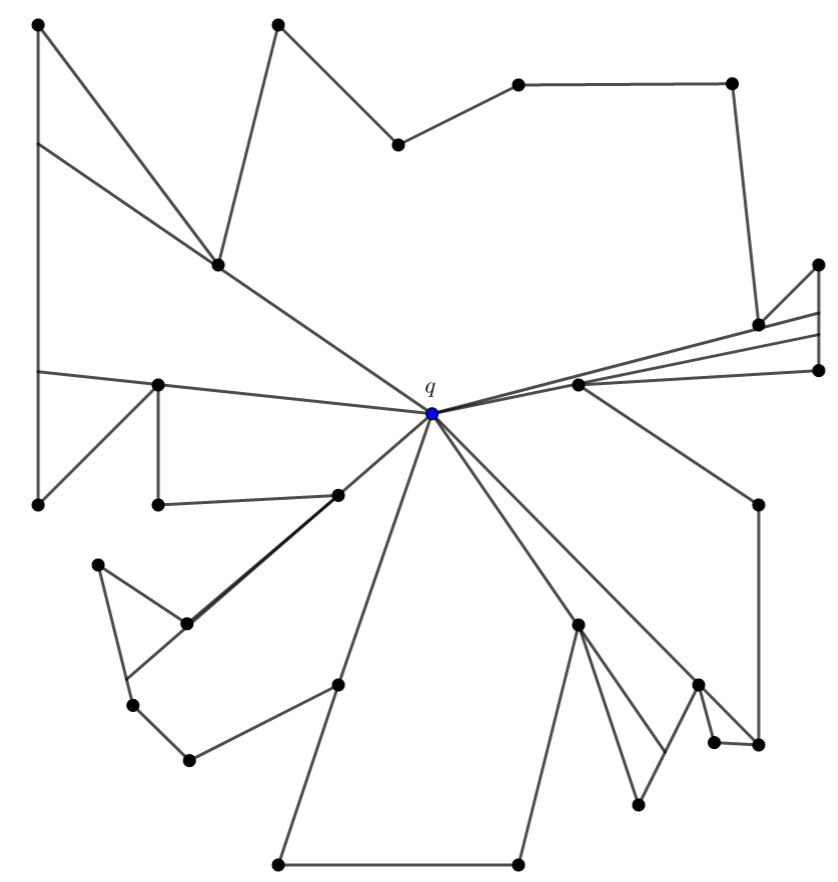
\includegraphics[width=0.55 \paperwidth]{images/V(q)09.png}
\end{frame}

\begin{frame}
  \centering 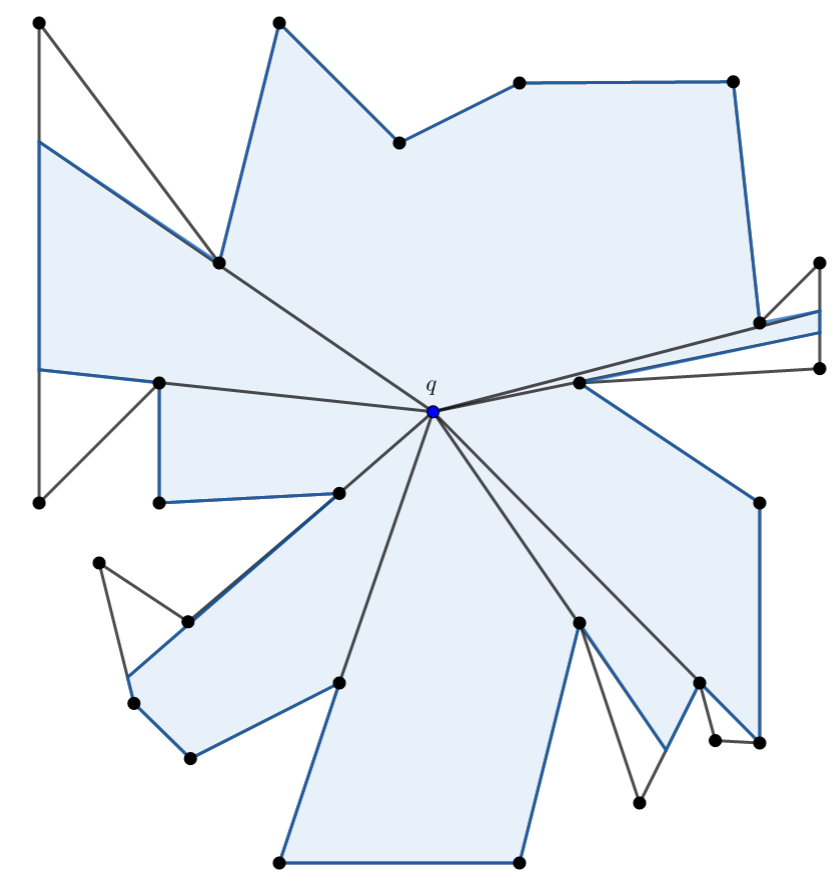
\includegraphics[width=0.55 \paperwidth]{images/V(q)10.png}
\end{frame}

\begin{frame}
  \centering 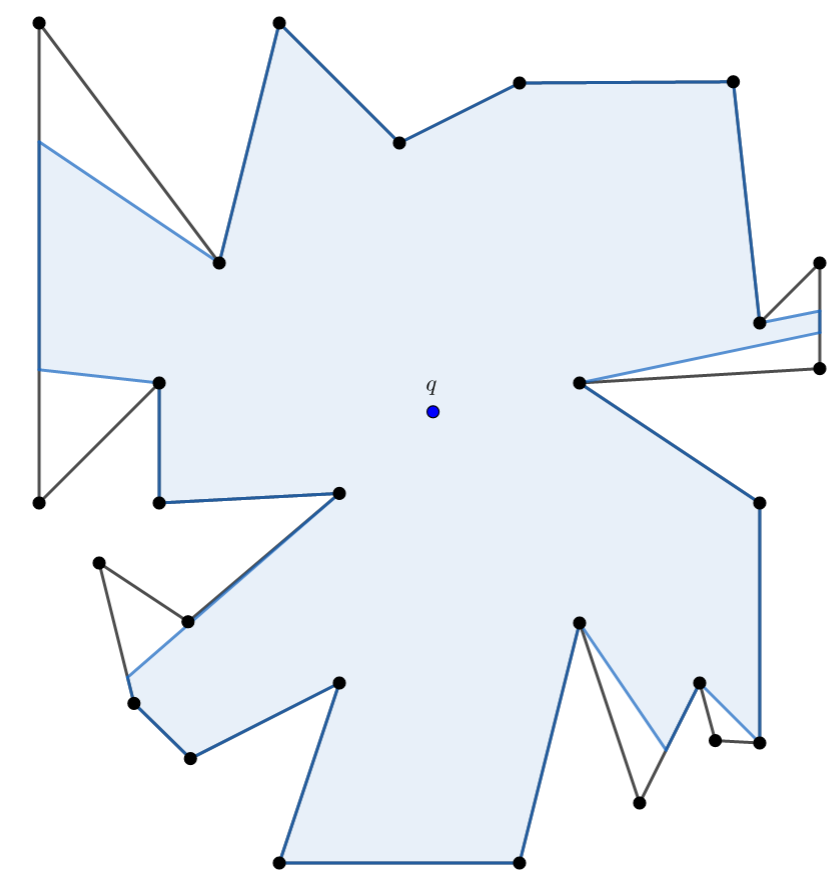
\includegraphics[width=0.55 \paperwidth]{images/V(q)11.png}
\end{frame}

\begin{frame}
  \frametitle{Introducción}
  En partícular, podemos tener distintos tipos de polígonos.
  
  \begin{figure}
    \centering
    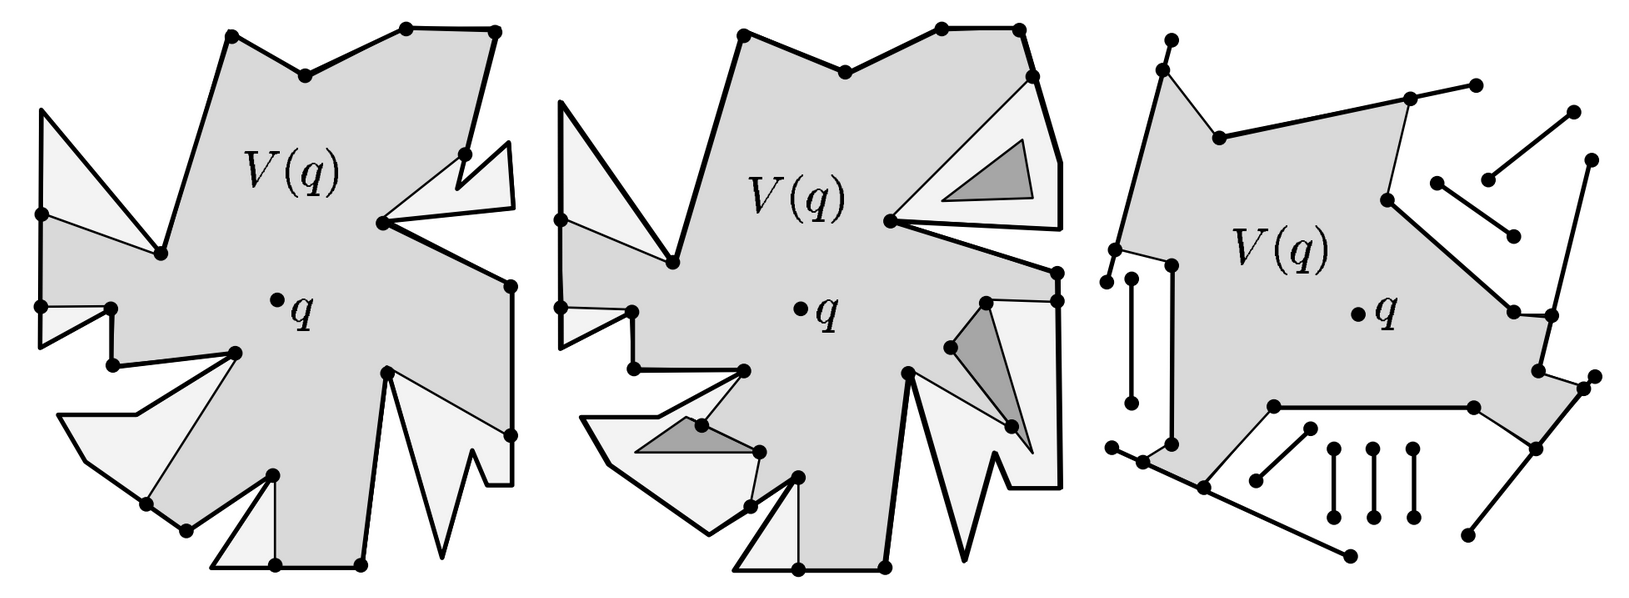
\includegraphics[width=0.75 \paperwidth]{./images/Casos.png}
    \caption*{Distintos casos para encontrar polígonos de visibilidad.}
  \end{figure}
  
  \textbf{Obs.} El polígono de visibilidad no, necesariamente, tiene que ser
  un polígono acotado.
\end{frame}
